\documentclass[a4paper,12pt]{article}

%%% Работа с русским языком
\usepackage{cmap}					% поиск в PDF
\usepackage{mathtext} 				% русские буквы в формулах
\usepackage[T2A]{fontenc}			% кодировка
\usepackage[utf8]{inputenc}			% кодировка исходного текста
\usepackage[english,russian]{babel}	% локализация и переносы

%%% Дополнительная работа с математикой
\usepackage{amsmath,amsfonts,amssymb,amsthm,mathtools} % AMS
\usepackage{icomma} % "Умная" запятая: $0,2$ --- число, $0, 2$ --- перечисление

%% Номера формул
%\mathtoolsset{showonlyrefs=true} % Показывать номера только у тех формул, на которые есть \eqref{} в тексте.
%\usepackage{leqno} % Нумерация формул слева

%% Свои команды
\DeclareMathOperator{\sgn}{\mathop{sgn}}

%% Перенос знаков в формулах (по Львовскому)
\newcommand*{\hm}[1]{#1\nobreak\discretionary{}
{\hbox{$\mathsurround=0pt #1$}}{}}

%%% Работа с картинками
\usepackage{graphicx}  % Для вставки рисунков
\graphicspath{materials}  % папки с картинками
\setlength\fboxsep{3pt} % Отступ рамки \fbox{} от рисунка
\setlength\fboxrule{1pt} % Толщина линий рамки \fbox{}
\usepackage{wrapfig} % Обтекание рисунков текстом

%%% Работа с таблицами
\usepackage{array,tabularx,tabulary,booktabs} % Дополнительная работа с таблицами
\usepackage{longtable}  % Длинные таблицы
\usepackage{multirow} % Слияние строк в таблице

%%% Теоремы
\theoremstyle{plain} % Это стиль по умолчанию, его можно не переопределять.
\newtheorem{theorem}{Теорема}[section]
\newtheorem{proposition}[theorem]{Утверждение}
 
\theoremstyle{definition} % "Определение"
\newtheorem{corollary}{Следствие}[theorem]
\newtheorem{problem}{Задача}[section]
 
\theoremstyle{remark} % "Примечание"
\newtheorem*{nonum}{Решение}

%%% Программирование
\usepackage{etoolbox} % логические операторы

%%% Страница
%\usepackage{extsizes} % Возможность сделать 14-й шрифт
\usepackage{geometry} % Простой способ задавать поля
	\geometry{top=25mm}
	\geometry{bottom=30mm}
	\geometry{left=25mm}
	\geometry{right=25mm}
 %

%%% Способ сделать тоже самое(но красивее:)
%\usepackage[margin=0.8in]{geometry}

 
\usepackage{fancyhdr} % Колонтитулы
 	\pagestyle{fancy}
 	\renewcommand{\headrulewidth}{0mm}  % Толщина линейки, отчеркивающей верхний колонтитул
 	\lfoot{}
 	\rfoot{}
 	\rhead{}
 	\chead{}
 	\lhead{ }
 	% \cfoot{Нижний в центре} % По умолчанию здесь номер страницы

\usepackage{setspace} % Интерлиньяж
%\onehalfspacing % Интерлиньяж 1.5
%\doublespacing % Интерлиньяж 2
%\singlespacing % Интерлиньяж 1

\usepackage{lastpage} % Узнать, сколько всего страниц в документе.

\usepackage{soulutf8} % Модификаторы начертания

\usepackage{hyperref}
\usepackage[usenames,dvipsnames,svgnames,table,rgb]{xcolor}
\hypersetup{				% Гиперссылки
    unicode=true,           % русские буквы в раздела PDF
    pdftitle={Заголовок},   % Заголовок
    pdfauthor={Автор},      % Автор
    pdfsubject={Тема},      % Тема
    pdfcreator={Создатель}, % Создатель
    pdfproducer={Производитель}, % Производитель
    pdfkeywords={keyword1} {key2} {key3}, % Ключевые слова
    colorlinks=true,       	% false: ссылки в рамках; true: цветные ссылки
    linkcolor=red,          % внутренние ссылки
    citecolor=green,        % на библиографию
    filecolor=magenta,      % на файлы
    urlcolor=blue           % на URL
}

%\renewcommand{\familydefault}{\sfdefault} % Начертание шрифта

\usepackage{multicol} % Несколько колонок

% Мои "дополнительные" пакеты
\usepackage{textcase} 
\usepackage{pdfpages}
\usepackage{amsmath}
\usepackage{titlesec}
\usepackage{floatrow}

\usepackage{subfig}

%% Делаем красивый header:
\fancyhead[RO]{\footnotesize{\scshape\nouppercase{~\leftmark}}}
%% Делаем красивый header END

%Делаем большой отступ между section и subsection
\titlespacing*{\section} {0pt}{3.5ex plus 1ex minus .2ex}{2.7ex plus .2ex}
\titlespacing*{\subsection} {0pt}{2.7ex plus 1ex minus .2ex}{1ex plus .2ex}


\begin{document} % конец преамбулы, начало документа

\begin{center}
	\textit{\MakeTextUppercase{федеральное государственное автономное учреждение}}
		
	\vspace{0.5ex}
	
	\textbf{ \\ \MakeTextUppercase{<<Московский Физико-технический институт>>}}
\end{center}
\vspace{13ex}
\begin{flushright}
	\noindent
	{Подкидышев Алексей}\\
	
	\textit{Студенты факультета инноваций\\ и высоких технологий\\(группа 792)}
\end{flushright}
\begin{center}
	\vspace{23ex}
	\line(1,0){430}\\[4ex]
	{\LARGE\textbf{Лабораторная работа 4.3}}
	\vspace{2ex}\\
	\textbf{\large{<<Изменение абсолютной активности препарата $^{60}Co$  методом $\gamma - \gamma$ совпадений>>}}\\[3ex]
	\line(1,0){430}\\[5ex]
	\vfill
	Долгопрудный 
	
	{\today}
\end{center}
\newpage
\renewcommand{\headrulewidth}{1pt}

% \section{Теоретическая часть}
\begin{multicols}{2}
[
\section{Теоретическая часть}
]



Определяется абсолютная активность радиоактивного препарата $^{60}Co$ с использованием каскадного перехода $\gamma$-квантов при его распаде. 
Закон радиоактивного распада:
	$$N=N_0e^{-\lambda t}$$
\par Абсолютная активность равна:
	$$N_0=\frac{4\pi m}{\varepsilon \omega}$$

где $\varepsilon$ - эффективность счетчика, $\omega$ -телесный угол.

\par
Описание $N_0$ значительно упрощается, если использовать в качестве образца радиоактивный элемент, при распаде которго последовательно испускаются несколько частиц.  Такие распады назваются каскадными. Распад $^{60}Co$ - каскадный.


Вероятность регистрации $\gamma$-кванта первым и вторым счетчиками:
$$P_1=\frac{\omega _1 \varepsilon _1}{4 \pi}$$
$$P_2=\frac{\omega _2 \varepsilon _2}{4 \pi}$$

Если включить оба счетчика в сему совпадений с разрешающим временем $\tau >> 10^{-11}$с, то каскадные $\gamma$-кванты будут регистрироваться одновременно. Вероятность совпадения будет равна:
	$$P_{\text{coвпадения}}=P_1P_2$$ 
Эта формула справедлива, если попадание одного $\gamma$-кванта  в первый счетчик и попадание второго во второй являются независимыми событиями. 
Вероятность истинных совпадений:
	$$P_{\text{coвпадения}}=W(\theta)P_1P_2$$ 
где $W(\theta)$ - корреляционная функция, определяющая анизотропию направления вылета второго $\gamma$-кванта по отношению к направлению первого. При $\theta = 180^{\circ}$ для $^{60}Co W=1.08$
Получаем для абсолютной активности выражение:
	$$N_0=1.08 \frac{N_1N_2}{2N_{co}}$$
где $N_1, N_2$ -истинные скорости счета, которые определяются как разность полной скорости счета и фона для каждого счетчика, а скорость истинных совпадений $N_{co}$ определяется как разность полного числа совпадений и числа случайных совпадений:
	$$n_c = 2 \tau n_1 n_2$$
где $\tau$ - разрешающее время схемы совпадений.
\end{multicols}

\begin{figure}[h!]
\centering
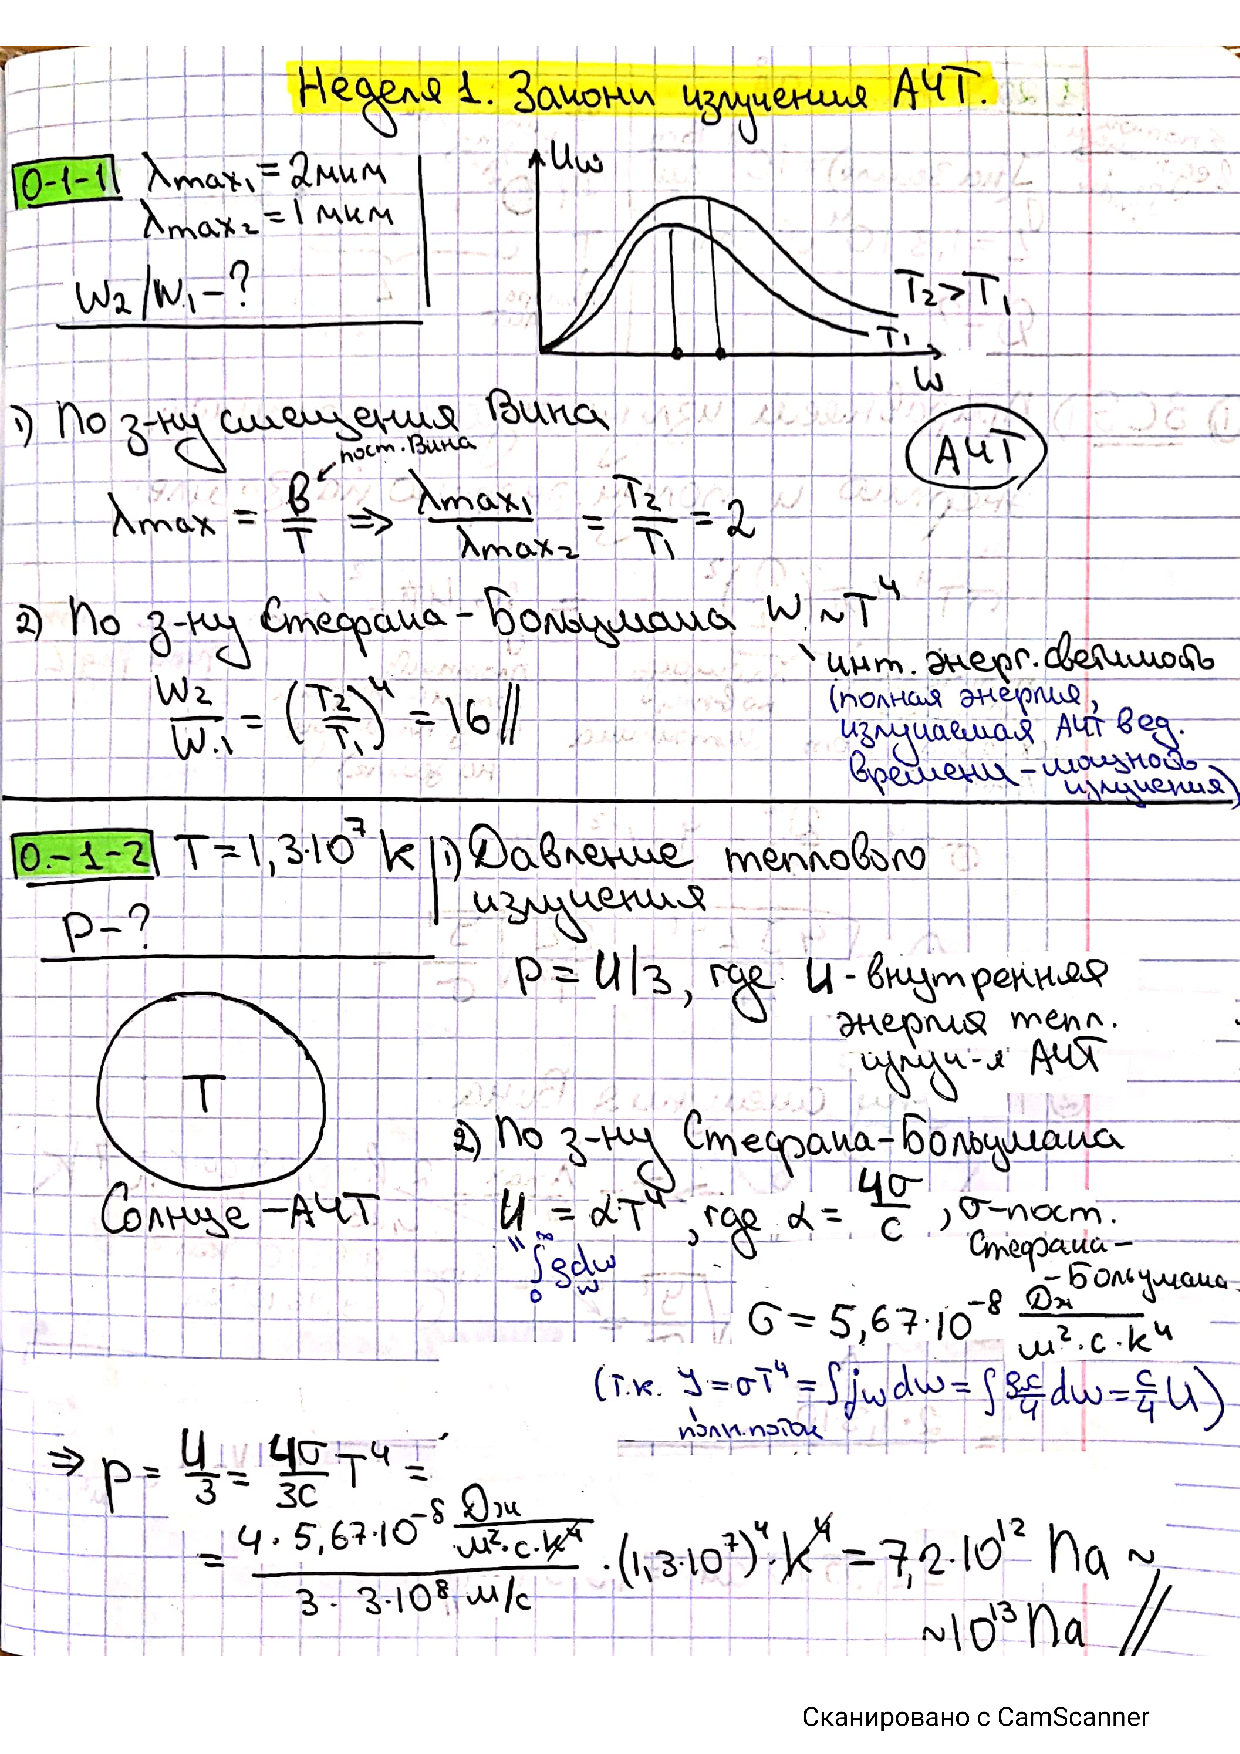
\includegraphics[scale=0.4]{1}
\caption{\textit{схема распада}} %уже есть
\end{figure} 

\section{Установка}

 \begin{figure}[H]
\centering
		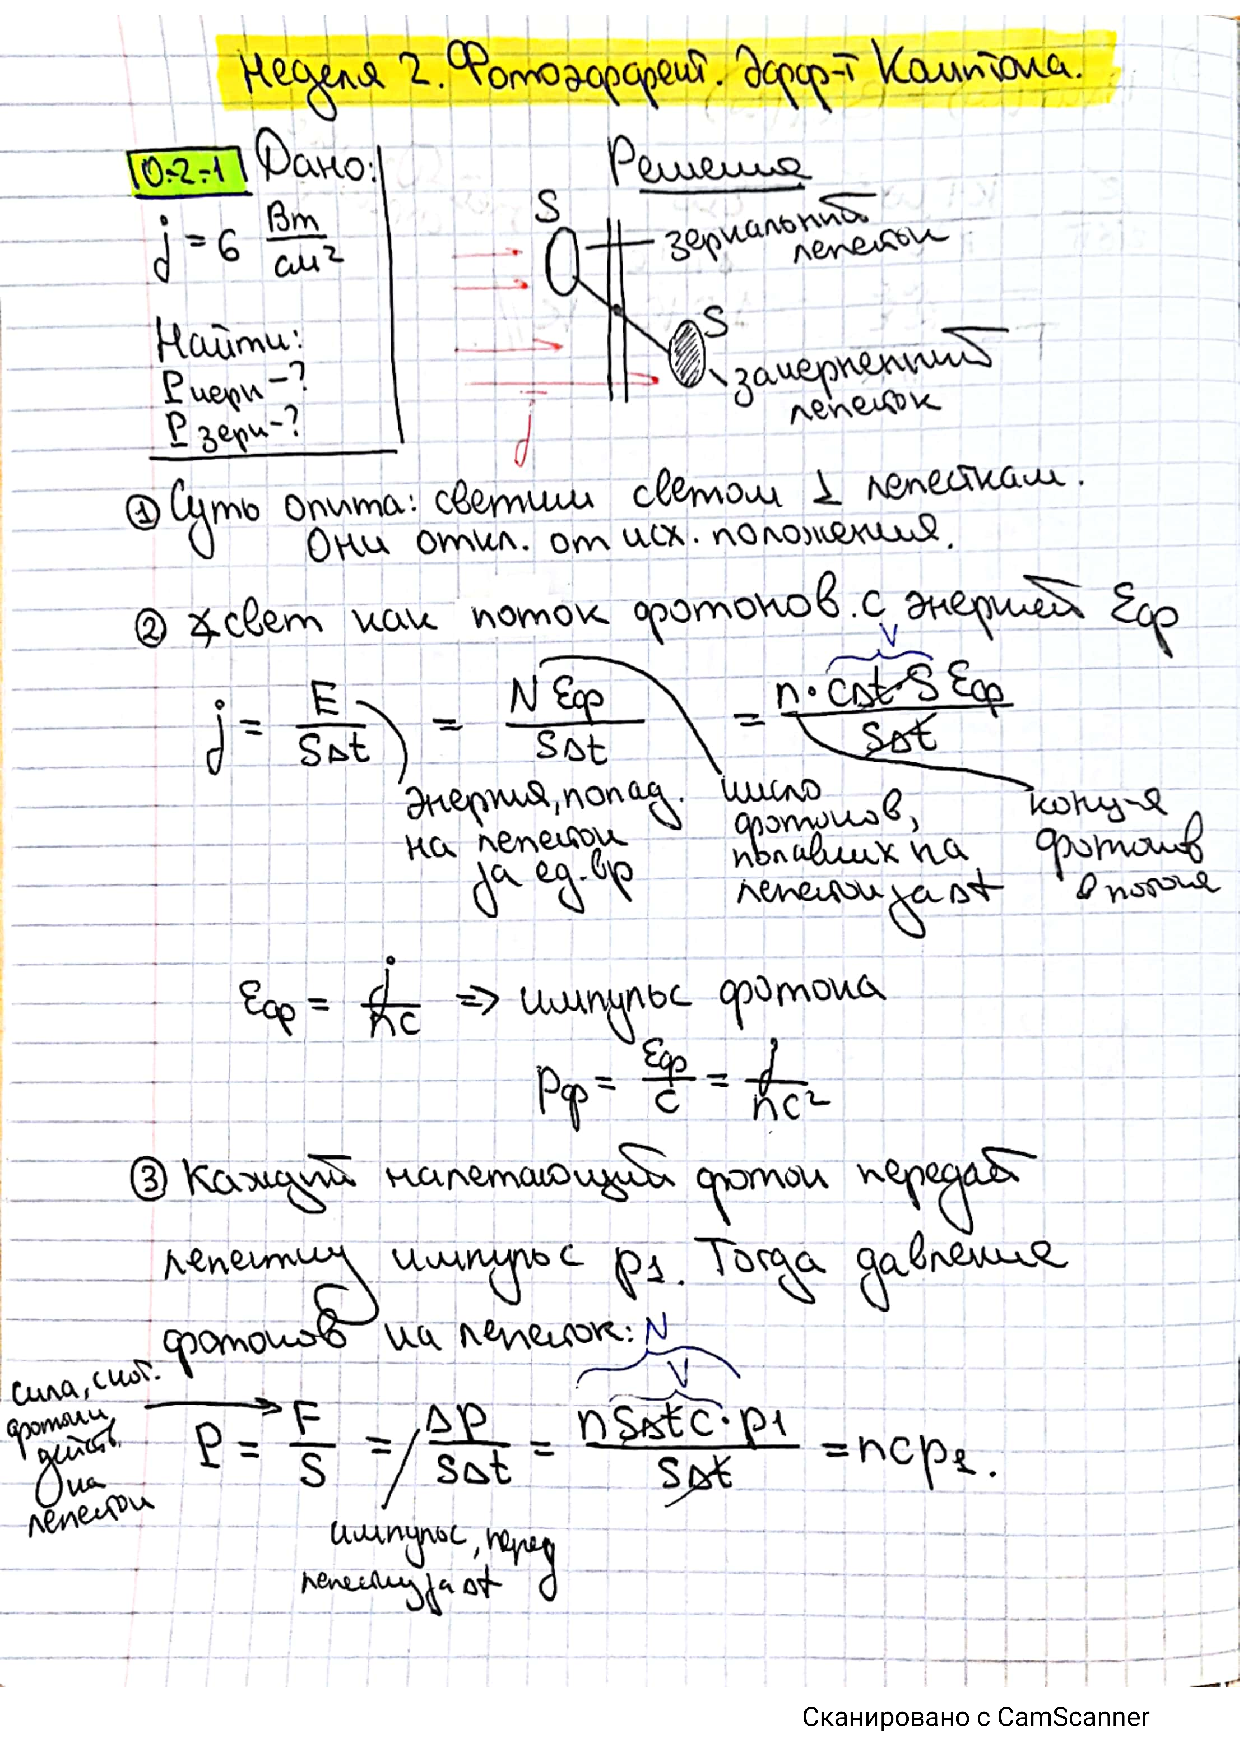
\includegraphics[scale=0.4]{2}
\caption{\textit{блок-схема установки}} % уже есть
\end{figure}

\section{Ход работы. Обработка результатов}

\begin{itemize}
    \item Определим фон для обоих источников. Занесем измерения в таблицу:
      
    \begin{table}[!h]
        \centering
            \begin{tabular}{ | c | c | c | c | c | c | c |}
                \hline
                \multicolumn{7}{| c |}{ФЭУ 1} \\ \hline
                $N_{\text{сч}}$ & 8699 & 8626 & 8663 & 8588 & 8504 & 8799 \\ \hline
                $N, \: \text{1 / с}$ & 145,0 & 143,8 & 144,4 & 143,1 & 141,7 & 146,6 \\ \hline
                $\langle N \rangle, \: \text{1 / с}$ & \multicolumn{6}{ c |}{144,1} \\ \hline
                \multicolumn{7}{| c |}{ФЭУ 2} \\ \hline
                $N_{\text{сч}}$ & 6362 & 6190 & 6450 & 6429 & 6341 & 6564 \\ \hline
                $N, \: \text{1 / с}$ & 106,0 & 103,2 & 107,5 & 107,2 & 105,7 & 109,4 \\ \hline
                $\langle N \rangle, \: \text{1 / с}$ & \multicolumn{6}{ c |}{106,5} \\ \hline
            \end{tabular}
        \caption{Результаты измерения фона для двух ФЭУ при времени счета $t = 1$ мин.} 
    \end{table}
    
    \item Измерим скорость счета $N_{1}$ в первом и $N_{2}$ во втором счетчиках(время счета $t = 1$ мин.):
        
    \begin{table}[H]
        \centering
            \begin{tabular}{ | c | c | c | c | c | c | c |}
                \hline
                \multicolumn{7}{| c |}{ФЭУ 1} \\ \hline
                $N_{\text{сч}}$ & 362572 & 365480 & 366234 & 368591 & 368652 & 367274 \\ \hline
                $N_{1}, \: \text{1 / с}$ & 6043,1 & 6091,5 & 6104,2 & 6143,2 & 6144,3 & 6121,7 \\ \hline
                $\langle N_{1} \rangle, \: \text{1 / с}$ & \multicolumn{6}{ c |}{6108,8} \\ \hline
                \multicolumn{7}{| c |}{ФЭУ 2} \\ \hline
                $N_{\text{сч}}$ & 342219 & 339444 & 339810 & 339011 & 339476 & 338554 \\ \hline
                $N_{2}, \: \text{1 / с}$ & 5704,6 & 5657,2 & 5664,3 & 5650,2 & 5658,5 & 5643,8 \\ \hline
                $\langle N_{2} \rangle, \: \text{1 / с}$ & \multicolumn{6}{ c |}{5662,5} \\ \hline
            \end{tabular}
        \caption{Результаты измерения скорости счета $\gamma$-квантов для двух ФЭУ при времени счета $t = 1$ мин.} 
        \label{tab:table_2}
    \end{table}
	
	\item Включим прибор в режим совпадений и измерим скорсти счета совпадений для различных разрешающих времен:
	
	\begin{table}[H]
        \centering
            \begin{tabular}{ | c | c | c | c | c | c | c |}
                \hline
                \multicolumn{7}{| c |}{$\tau = 100 \: ns$} \\ \hline
                $N_{\text{сч}}$ & 567 & 532 & 525 & 528 & 568 & 521 \\ \hline
                $N_{\text{совп}}, \: \text{1 / с}$ & 9,4 & 8,9 & 8,8 & 8,8 & 9,5 & 8,7 \\ \hline
                $\langle N_{\text{совп}} \rangle, \: \text{1 / с}$ & \multicolumn{6}{ c |}{9,0} \\ \hline
                \multicolumn{7}{| c |}{$\tau = 200 \: ns$} \\ \hline
                $N_{\text{сч}}$ & 1107 & 1075 & 1078 & 1096 & 1052 & 1162 \\ \hline
                $N_{\text{совп}}, \: \text{1 / с}$ & 18,4 & 17,9 & 18,0 & 18,3 & 17,5 & 19,4 \\ \hline
                $\langle N_{\text{совп}} \rangle, \: \text{1 / с}$ & \multicolumn{6}{ c |}{18,3} \\ \hline
                \multicolumn{7}{| c |}{$\tau = 500 \: ns$} \\ \hline
                $N_{\text{сч}}$ & 2263 & 2297 & 2493 & 2291 & 2308 & 2294 \\ \hline
                $N_{\text{совп}}, \: \text{1 / с}$ & 37,7 & 38,3 & 41,6 & 38,2 & 38,5 & 38,2 \\ \hline
                $\langle N_{\text{совп}} \rangle, \: \text{1 / с}$ & \multicolumn{6}{ c |}{38,7} \\ \hline
            \end{tabular}
        \caption{Результаты измерения скорости счета $\gamma$-квантов для двух ФЭУ при времени счета $t = 1$ мин.} 
        \label{tab:table_3}
    \end{table}
    
\item Построим график зависимости $N_0$ от разрешающего времени $\tau$:
\begin{figure}[H]
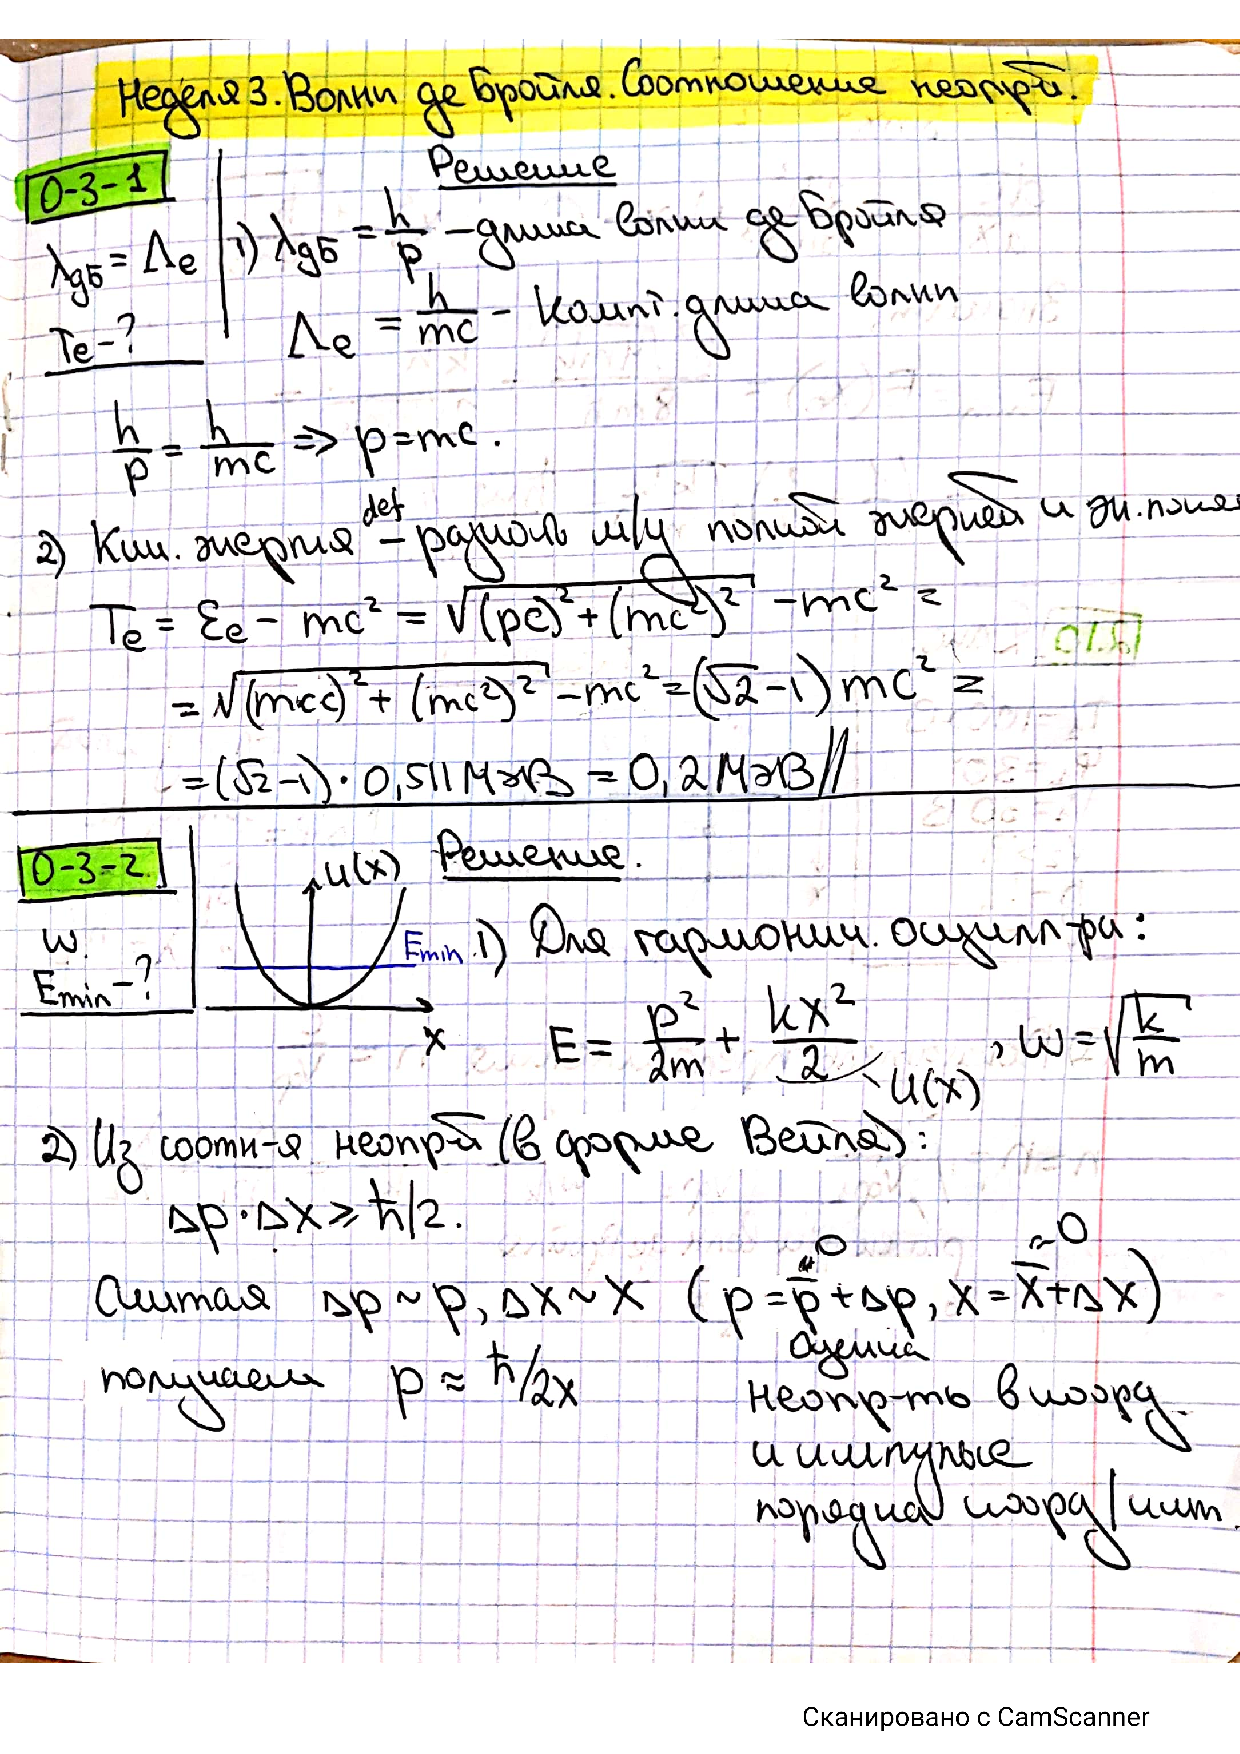
\includegraphics[scale=0.5]{3}
\caption{График зависимости абсолютной активности источника $^{60}\text{Co}$ от разрешающего времени схемы совпадений $\tau$.}
\end{figure}
	
\end{itemize}

\section{Вывод}
\begin{enumerate}
    \item Определили активность радиоактивного препарата: $^{60}\text{Co}$.
    \item  Получили  зависимость абсолютной активности препарата от разрешающего времени схемы совпадений.
\end{enumerate}{}

\end{document}